\documentclass[10pt,conference,compsocconf]{IEEEtran}
%\documentclass[journal]{IEEEtran}
\usepackage{amsmath, amsthm, amsfonts, amssymb}
\usepackage{graphicx}

\usepackage{multirow}
\usepackage{enumerate}
\usepackage[table,xcdraw]{xcolor}
\usepackage{amsmath}
\usepackage{diagbox}
\usepackage{bm}
\usepackage{algorithmic,algorithm}
\usepackage{etoolbox}
\usepackage{color,xcolor}
\usepackage{booktabs}
%\usepackage{caption}
\usepackage{subcaption}
\usepackage{hyperref}
%\usepackage{gensymb}

\usepackage{array}
\usepackage{makecell}

\renewcommand\theadalign{bc}
\renewcommand\theadfont{\bfseries}
\renewcommand\theadgape{\Gape[1.5pt]}
\renewcommand\cellgape{\Gape[1pt]}
\newcommand{\wz}{{\color{white}0}}

\renewcommand{\arraystretch}{1.25}


\begin{document}
\title{Open and Closed loop Trajectory Planning --Semester project report}

\author{
Yifeng Chen, Supervisor: Kaouther Messaoud Ben Amor, Professor: Alexandre Alahi\\
  \textit{\'Ecole Polytechnique F\'ed\'erale de Lausanne, Switzerland}
}

\maketitle

\section{Introduction} \label{sec:Introduction}
In the last few years,
larg-scale human labeled datasets combined with Deep Neural Networks have led to a significant performance increase in autonomous vehicle perception. While there is a growing body of ML-based motion planners, the lack of simulation frameworks and metrics has limited the progress in this area. 

Existing benchmarks (Argoverse, Lyft, Waymo) for autonomous vehicle motion prediction have focus on short term motion forecasting of other agents rather than long-term planning of the ego vehicle, which has led previous works to use open-loop evaluation with L2-based metrics, which are not appropriate for fairly evaluating long-term planning. Nuplan benchmarks overcomes these limitations by providing a training framework to develop machine learning based planners, a lightweight open-loop and closed-loop simulator, motion-planning specific metrics and an interactive visualization tool.

In this project, based on nuplan benchmarks, 3 neural networks (Raster model, LaneGCN model and Vision transformer model) are built in order to train a planner for solving autonomous vehicle planning problem. A high quality dataset with 1500h of human driving data from 4 cities across the US and Asia with widely varying traffic patterns is considered to train the planner and simulate the real scenario. 2 simulation methods (open-loop and closed-loop) are considered to simulate the real scenarios. Several metrics from open-loop and closed-loop are considered to evaluate each method. Finally, all planners' predicting results are visualized and compared.


\section{Related work}
In this section, the nuPlan framework, simulation tasks as well as previous ML-based planning methods will be discussed

\subsection{nuPlan framework}

As shown in Table \ref{tab:nuPlan}, nuPlan dataset and relevant prediction datasets are compared.\cite{nuplan} nuPlan Dataset has the largest data size (1500 driving hours in 4 cities). Except the nuPlan datasets, the other dataset focus on predicting rather than planning. Besides, nuPlan dataset contains Sensor Data. Finally, its evaluation method considers both open-loop and closed-loop metrics.

\begin{table}[h]
    \centering
    \begin{tabular}{c|c|c|c|c|c}
       Dataset  & Data & Cities & Sensor Data & Type & Evaluation \\
       \hline
        Argoverse & 320h & 2 & & Pred & OL \\
        nuPredict & 5h & 2 & \checkmark & Pred & OL \\
        Lyft & 1118h & 1 & & Pred & OL \\
        Waymo & 570h & 6 & & Pred & OL \\
        nuPlan & 1500h & 4 & \checkmark & Plan & OL+CL
        
    \end{tabular}
    \caption{A comparison between motion prediction (Pred) and planning (Plan). dataset size, number of cities, availability of sensor data, dataset type, and evaluation methods are shown here.}
    \label{tab:nuPlan}
\end{table}



\subsection{Simulation tasks}

\subsubsection{Open-loop}
In the open-loop simulation task, the goal of planning system is to imitate a human driver. For every timestep, the trajectory is scored based on displacement or heading difference metrics, which is not used to control the vehicle. Therefore, no interaction is considered.

In this task, average heading error (AHE), final heading error (FHE), average displacement error (ADE) and final displacement error (FDE) are considered.

\subsubsection{Closed-loop}

In the closed-loop simulation task, the planner outputs a planned trajectory using the information available at each time step, similar to the open-loop simulation task. However, the proposed trajectory is regarded as a reference and thus, the planning system is corrected at each time step with the new state of the vehicle.

In this task, drivable area compliance, minimun time to collision, the progress ratio between ego and expert and comfortable metrics are considered. 

\subsection{Previous ML-based planning methods}

In this subsection, 2 models are introduced and their strengths and limitations are compared.


\subsubsection{LaneGCN model}

As shown in Figure\ref{fig:LaneGCN}, the architecture of LaneGCN consists of 4 modules\cite{LaneGCN}: ActorNet, MapNet, FusionNet and prediction header. 1. \emph{ActorNet} takes the past actor trajectories as input, and uses 1D convolution to extract actor node features. 2. \emph{MapNet} builds a lane graph from HD maps, and uses a LaneGCN to extract lane node features. 3. \emph{FusionNet} contains 4 interaction blocks. The actor to actor block fuses real-time traffic information from actor nodes to lane nodes. The lane to lane block processes information over the lane graph and renews lane features. The actor to actor block performs interactions among actors. Another LaneGCN is applied for the lane to lane block, and spatial attention layers are applied for the other blocks. 4. The \emph{prediction header} uses after-fusion actor features to create multi-modal trajectories.
\subsubsection{Raster model}

Raster-based model that uses a CNN backbone to encode ego, agent and map information as raster layers.\cite{Raster} Any pretrained backbone from the TIMM library can be used (e.g. ResNet50, EfficientNetB3).

\subsubsection{Comparison between 2 models}

\begin{itemize}
    \item \emph{Input information}:
(1) the inputs of \emph{LaneGCN} contains 2 parts: Vector map data and Agents information. Vector map data contains coordinates, grouping information of each lane, on-route status, and traffic light status. Agents information contains the status (x, y, heading) of ego and surrounding 
vehicles in 5 frames. (2) the inputs of \emph{Raster} is a 4-dimension image, they are ego, agent, baseline path and Roadmap layer. Therefore, we could see the input of \emph{LaneGCN} contains more temporal information as well as more road status information, while \emph{Raster} contains more map spatial information.

\item \emph{Graph construction difference}: (1) For Raster model, it considers the map as a rasterized map, which fuses with LiDAR point clouds to perform joint perception and prediction as well as end-to-end motion planning. However, since it applies CNN backbone, it could only capture local information from the map. (2) For LaneGCN model, it regards map as a VectorNet, which could capture multi-scale topology features, and it could also model global interactions between actor and lane features.
\end{itemize}












\begin{figure}[!ht]
	\centering
	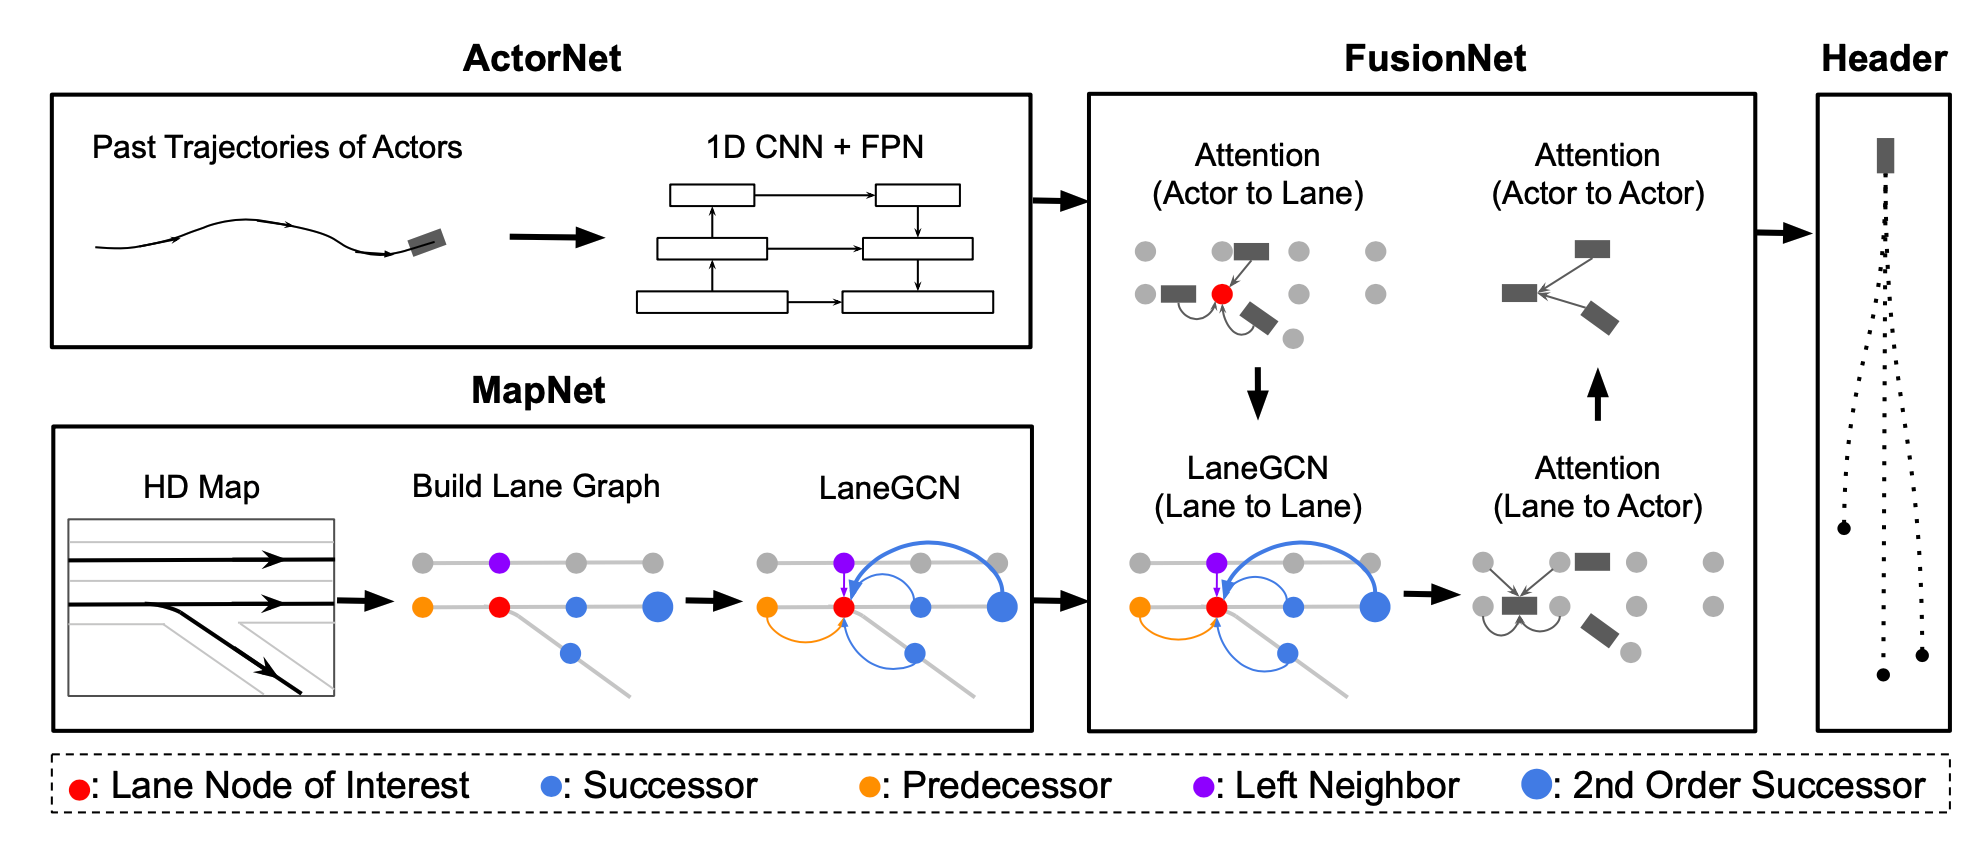
\includegraphics[width=0.9\linewidth]{LaneGCN.png}
	\caption{The architecture of LaneGCN}
    \label{fig:LaneGCN}
\end{figure}

\section{Method Implementation}

\subsection{Vision Transformer}
The architechture of Vision Transformer (VIT) is shown in Figure\ref{fig:VIT}, An image is splited into fixed-size patches, linearly embed each of them, add position embeddings, and feed the resulting sequence of vectors to a standard Transformer encoder. By applying adding an extra learnable classification token to the sequence, it could perform classification.\cite{VIT}

\begin{figure}[!ht]
	\centering
	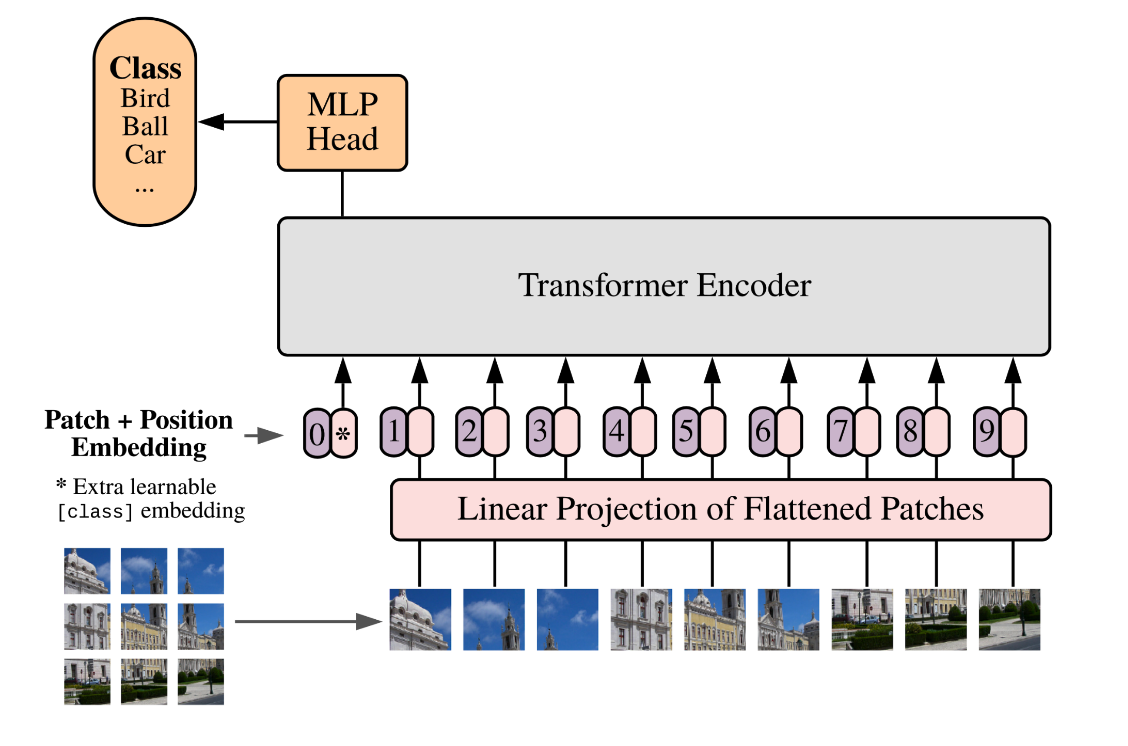
\includegraphics[width=0.9\linewidth]{VIT.png}
	\caption{The architecture of VIT}
    \label{fig:VIT}
\end{figure}
\subsection{Input and Output}

From Figure \ref{fig:VITIO}, the input and output of VIT are shown in the graph. The input is an image, consisting of 4 layers, which are Ego agent, surrounding agent, baseline path and roadmap layer information. The output is a ego's trajectory, consisting of x, y, heading information in next 8 seconds, the time interval of it is 0.5 second.


\begin{figure}[!ht]
	\centering
	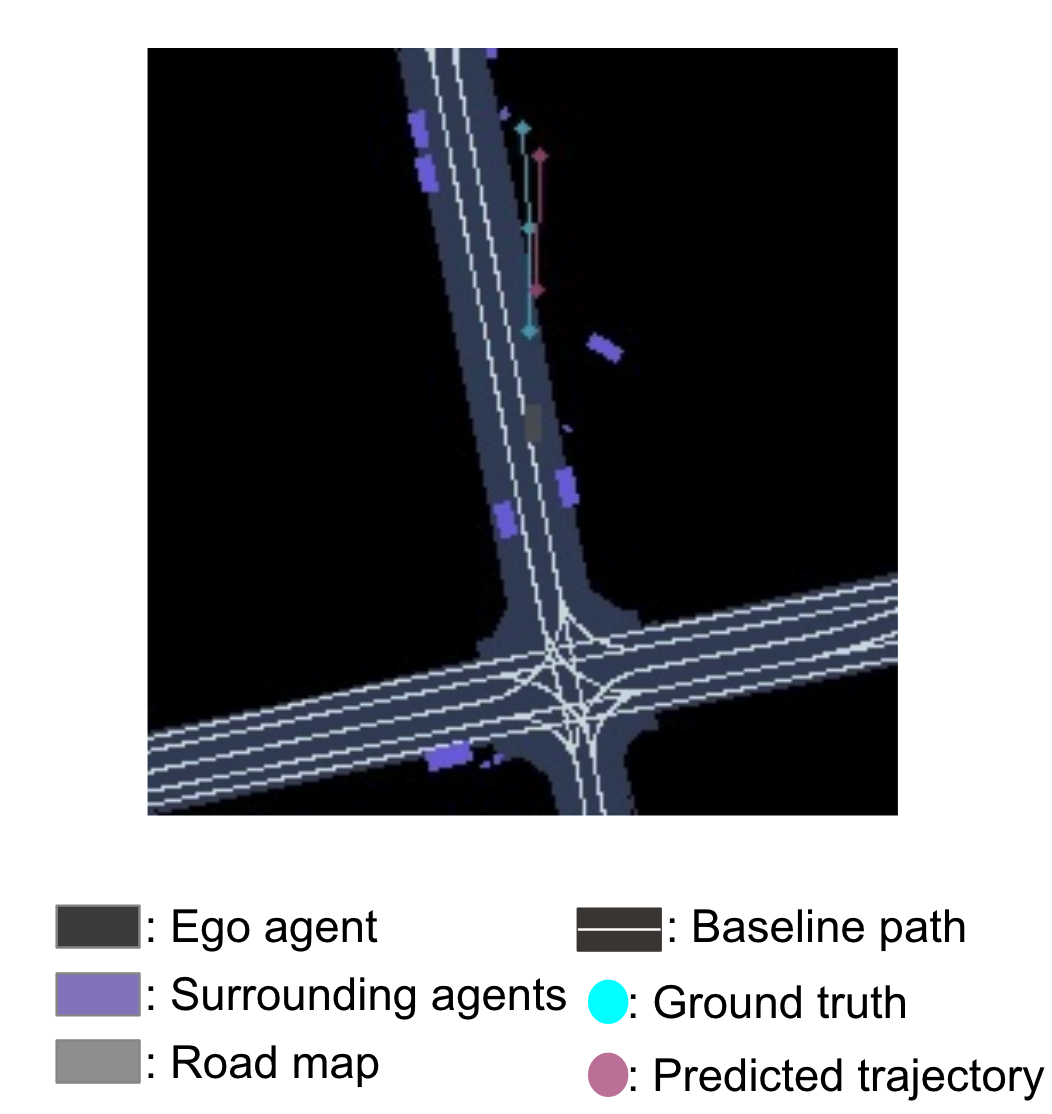
\includegraphics[width=0.9\linewidth]{VITIO2.png}
	\caption{The input and output of VIT}
    \label{fig:VITIO}
\end{figure}
\subsection{Loss Function}
The loss is a weighted loss, which is divided into 2 parts, one part is for calculating the loss of coordinates by using MSE loss, another part is for calculating the loss of heading by using L1 loss.

The formula is shown in eq.\ref{eq:1}
\begin{equation}
    \begin{align}
        min\space w_1[(target_x-predict_x)^2+
        \\(target_y-predict_y)^2]+
        \\
        w_2|target_{heading}-predict_{heading}|
    \end{align}
    \label{eq:1}
\end{equation}
\section{Experiments}
\subsection{Dataset description}
\subsubsection{Overview}

1500 hours of data from Las Vegas, Boston, Pittsburgh, and Singapore are released. Each city provides its specific driving challenges. For example, Boston routes include drivers who love to double park, Singapore features left hand traffic. Semantic maps and an API for efficient map queries were provided for eac
h city. Besides, Lidar point clouds, localization information, camera images and steering inputs are included.

\subsubsection{Scenarios}

Intervals with tags for complex scenarios are annotated automatically in order to enable scenario-based metrics. These scenarios include lane changes, merge, protected or unprotected left or right turns, interaction with 
cyclists, interaction with pedestrians or cyclists, double parked vehicles, stop controlled intersections and driving in construction zones.
\subsection{Results analysis}
\subsubsection{Metrics Comparison}
Based on the open-loop and closed-loop simulation, several metrics are tested and compared, which could be found in the table \ref{tab:open-loop}
\ref{tab:Closed-loop}

From the open-loop metrics, it could be found that  the LaneGCN has the best performance in ADE and FDE, raster model has the best performance in AHE and FHE, the result of VIT model seems not ideal
From the closed-loop metrics, it could be found that  Raster model has the best performance, VIT model has a better performance compared to LaneGCN model.

\begin{table}[h]
    \centering
    \begin{tabular}{c|c|c|c|c}
        Model & ADE & AHE & FDE & FHE \\
        \hline
        LaneGCN & 4.817&0.1113&11.01&0.2158\\
        Raster & 12.77 & 0.1009 & 24.53 & 0.1686 \\
        VIT& 14.82& 0.1921&27.64&0.3246
    \end{tabular}
    \caption{Open-loop Metrics comparison between different models
}
    \label{tab:open-loop}
\end{table}
\begin{table}[h]
    \centering
    \begin{tabular}{c|c|c|c|c}
       Model  & Drivable area  & Min
       time  & Ego expert   & Ego is 
       \\
       &compliance&to collision&
       progress ratio&comfortable\\
       \hline
        LaneGCN & 0& 0.2 & 0.471 & 0.25\\
        Raster & 0.8 & 0.625 & 0.389 & 0.625\\
        VIT & 0.55 & 0.35 & 0.517 & 0.275
    \end{tabular}
    \caption{Closed-loop Metrics comparison between different models
}
    \label{tab:Closed-loop}
\end{table}
\subsubsection{Scenario Comparison}
3 scenarios are also picked and compared, which could be found in Figure \ref{fig:Scenario Comparison} It could be seen that for first scenario, all of them have a great performance. For the second scenario, it could be seen that the LaneGCN has a best performance, then is raster, and VIT’s performance seems not ideal. For the last scenrio, it could be seen that all of them don’t have an ideal result, but LaneGCN and Raster could learn the scenario boundary information.


\begin{figure}[!ht]
	\centering
	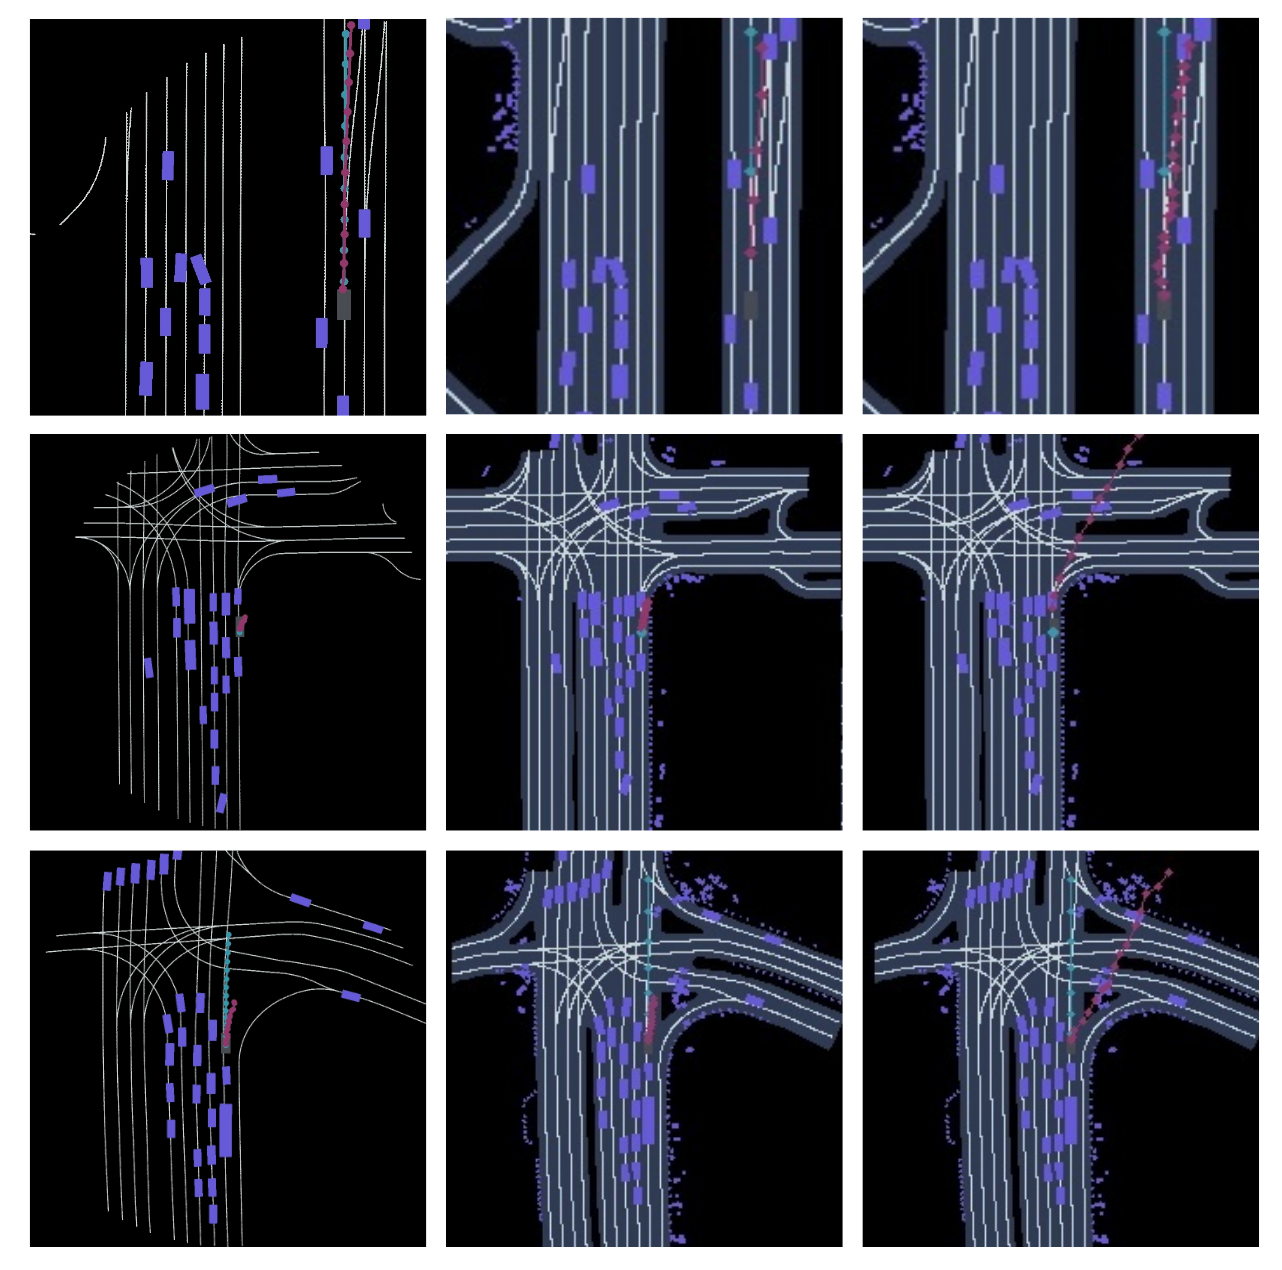
\includegraphics[width=0.9\linewidth]{Scenarios Comparison.png}
	\caption{Scenarios Comparison. 
 \emph{left}: LaneGCN, \emph{middle}: Raster, \emph{right}:VIT, \emph{upper}: Going straight, \emph{middle}: Stopping, \emph{bottom}: going straight (intersection)
}

    \label{fig:Scenario Comparison}
\end{figure}
\section{Conclusion }
In this semester project, the nuplan framework is implemented and 3 models are trained and the results are compared. The LaneGCN and Raster model still have a better performace in different scenairos and in the open-loop simulation. However, the VIT model has a great performance in closed-loop simulation, which proves its potential ability for planning. 

In the future, Multiple frames could be considered as input and pretrained weights could be applied for training. 













\bibliographystyle{IEEEtran}
\bibliography{literature}






\end{document}
